We will find the current response of a single Dirac cone, with a temperature gradient $\nabla_y T$ and a magnetic field $B_z$.
The current response of interest in the given geometry is thus in the $x$-direction,
\begin{equation}\label{eq:3}
  J^x = \chi ^{xy} \frac{- \nabla _yT}{T},
\end{equation}
with $\chi^{xy}$  being the response\footnote{The sign in Eq. (\ref{eq:3}) depends on the choice of the response function being the response of the gravitational potential or the temperature gradient. Thus, the sign may differ in the literature.}.
This geometry is shown in Figure \ref{fig:setup}.
\begin{figure}[ht]
  \centering
  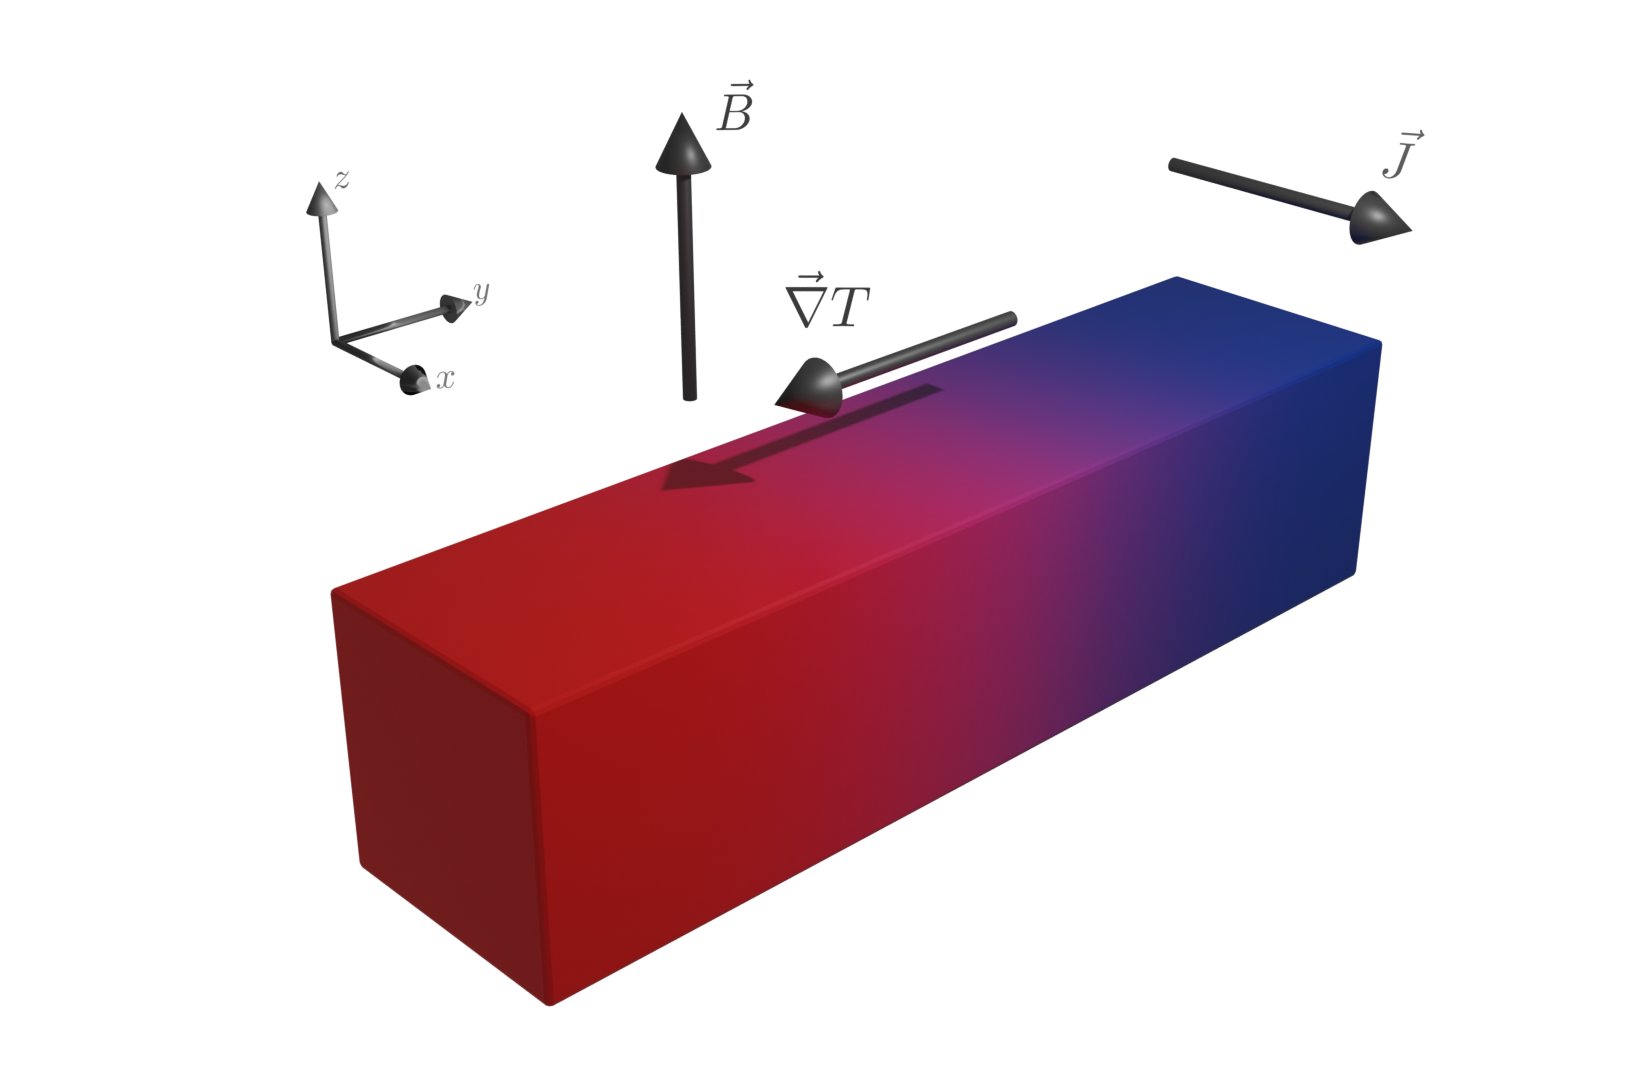
\includegraphics[width=0.7\textwidth]{figures/setup.png}
  \caption{Sketch of the geometry used in the derivation. Note that we consider only bulk response, and the finite sample is only for illustration purposes. \label{fig:setup}}
\end{figure}
In the derivation of~\citeauthor{chernodubGenerationNernstCurrent2018}~\cite{chernodubGenerationNernstCurrent2018} the response
\begin{equation}
  \chi ^{xy} = \frac{e^2 v_F B}{18 \pi ^2 \hbar }
\end{equation}
was found, while the derivation of~\citeauthor{arjonaFingerprintsConformalAnomaly2019}~\cite{arjonaFingerprintsConformalAnomaly2019} found
\footnote{The paper is somewhat unclear on what is their final result, as there is some possible confusion related to the number of Landau levels included and whether one is including both or only one Dirac cone.
The above result is what is meant, to the best of our understanding.}
\begin{equation}
  \chi ^{xy} = \frac{e^2 v_F B}{4 \pi ^2 \hbar }.
\end{equation}

Recall the linear response from the Kubo formalism in Eq. (\ref{eq:current-luttinger-gravity-final}), found through Luttinger's approach.
\begin{equation}
  \label{eq:4}
  \braket{J^i}(t, \vec{r}) =
  \int\limits_{-\infty }^{\infty } \mathrm{d}t' \mathrm{d}\vec{r}'
  \int\limits_{-\infty }^{t'} \mathrm{d}t''
  \left\{
    \frac{-i v_F}{\hbar } \Theta (t-t')
    \Braket{
      [J^i(t, \vec{r}), T^{0j} (t'', \vec{r}')]
    }
  \right\}
  \partial _j' \psi (t', \vec{r}').
\end{equation}
Fourier transforming now to the frequency and momentum domain, will be beneficial in our calculations.
As before, the non-perturbed system will be taken to be time and position invariant, such that the correlator in Eq. (\ref{eq:4}) can be taken to depend only on the differences $t-t''$ and $\vec{r} - \vec{r}' $.
Starting with Fourier transforming the position part, notice that the structure of Eq. (\ref{eq:4}) is
\[
  \braket{J^i}(\vec{r}) = \int \mathrm{d} \vec{r}' \chi (\vec{r} - \vec{r}') \partial _j' \psi  (\vec{r}'),
\]
where the temporal parts were dropped for clarity.
This is a convolution, and the Fourier transform is thus simply given by the product of the two factors~\cite{rottmannMatematiskFormelsamling1995}.
\begin{equation}
  \braket{J^i}(\vec{q}) =
  \chi (\vec{q}) (iq_j) \psi (\vec{q}),
\end{equation}
where it was also used that the Fourier transform of a derivative gives the component of the variable.
Showing explicitly how to find the form of the response $\chi $ in momentum space is often overlooked in much literature, and as it does involve some finesse, we want to show it here.
This trick is courtesy of~\citeauthor{changLectureNotesManybody2018}~\cite{changLectureNotesManybody2018}.
By definition, the Fourier transform of the response is, where the variable of integration has been chosen to be $\vec{r}-\vec{r}'$ for later convenience,
\begin{align}
  \chi (\vec{q}) &= \int \mathrm{d}(\vec{r} - \vec{r}') e^{-i\vec{q}(\vec{r}-\vec{r}')} \chi (\vec{r} - \vec{r}')\\
                 &= \int \mathrm{d}(\vec{r} - \vec{r}') e^{-i\vec{q}(\vec{r}-\vec{r}')} C \Braket{
                   \left[
J^i (\vec{r}), T^{0j}(\vec{r}')
                   \right]},\\
\end{align}
where $C$ denotes $t$-dependent prefactors and integrals over time are omitted, again for clarity of notation.
Note that
\begin{equation}
  \int \mathrm{d}(\vec{r} - \vec{r}') = \frac{1}{\mathcal{V}} \int \mathrm{d}\vec{r} \mathrm{d} \vec{r}',
\end{equation}
where $\mathcal{V}$ is the volume of the system.
Thus,
\begin{equation}
  \begin{split}
    \chi (\vec{q}) &= \frac{1}{\mathcal{V}} \int \mathrm{d}\vec{r} \mathrm{d}\vec{r}'
    e^{-i\vec{q}(\vec{r}-\vec{r}')}
    C \Braket{\left[
        J^i(\vec{r}), T^{0j}(\vec{r}')
      \right]}\\
    &= \frac{C}{\mathcal{V}} \Braket{\left[ J^i(\vec{q}), T^{0j}(-\vec{q}) \right]}.
  \end{split}
\end{equation}

Considering now the temporal part, the procedure is simpler.
The linear response still has the form of a convolution, as the response function is only dependent on the difference $t-t'$ by
\begin{equation}
  \chi (t-t') = \int\limits_{-\infty }^0 \mathrm{d} t'' \Theta (t - t')
  \Braket{\left[ J(t-t'), T(t'') \right]},
\end{equation}
where $t''$ was shifted by $t' $, and then the translational invariance of the correlator was used.
In frequency space
\begin{align}
  \chi (\omega ) &= \int \mathrm{d} t e^{i \omega  t} \chi (t)\\
                 &= \int \mathrm{d} t e^{i \omega  t} \int\limits_{-\infty  }^0 \mathrm{d} t''
                   \Theta (t) \Braket{\left[ J(t), T(t'') \right]}.
\end{align}
In frequency and momentum space the response function is thus
\begin{equation}\label{eq:5}
  \chi ^{ij} (w, \vec{q}) =
  \frac{-iv_F}{\mathcal{V} \hbar }
  \int \mathrm{d}t e^{i\omega t}
  \int\limits_{-\infty }^{0} \mathrm{d}t'
  \Theta (t)
  \Braket{\left[
      J^i(t, \vec{q}), T^{0j}(t', -\vec{q})
    \right]}.
\end{equation}

\subsection{Transport and magnetization}
Recall that we generally define the transport coeffieicents
\[
J^i = e^2 L^{ij}_{11} E_j + e L_{12}^{ij} \nabla_jT,
\]
where \( J^i \) is the electrical current.
In our work, we focus on the \( L_{12} \) coefficient, however the following discussion is valid also more generally.
The definition of transport currents becomes more subtle in systems with broken time-reversal symmetry\cite{vanderwurffMagnetovorticalThermoelectricTransport2019, chernodubThermalTransportGeometry2021}.
In such systems, unobservable, circulating \emph{magnetization} currents arise.
These currents do not contribute to transport, but the Kubo treatment derives the local current, which in general also includes non-transporting currents.
Let
\begin{equation}
  \label{eq:1}
  \vec{J} = \vec{J}_{\text{tr}} + \vec{J}_M,
\end{equation}
where \( \vec{J} \) is the total local current, \( \vec{J}_{\text{tr}} \) is the transport current, and \( \vec{J}_M \) is the circulating magnetization current.
While our response \( \chi \) relates to the total current, we are more interested in the experimentally measurable transport resonse \( L^{ij}_{12} \), related to our Kubo result as \cite{arjonaFingerprintsConformalAnomaly2019}
\todo{this might not be a first-hand source. See thermal transport...geometry chernodub eq. 62}
\begin{equation}
  \label{eq:2}
  L_{12}^{ij} = \chi^{12} - \epsilon^{ijl} M_l,
\end{equation}
with \( M_l \) the magnetization.
For zero chemical potential, however, these magnetization currents have been shown to go to zero as \( T \to 0 \).
